
\chapter{Plan de développement}

\section{Planning}

\par
La figure \ref{gantt} (page \pageref{gantt}), montre le planning prévisionnel pour l'ensemble du projet.
Le détail de chaque tâche est spécifié dans la section suivante.

\begin{figure}[p]
\vspace*{-2.5cm}
\centerline{
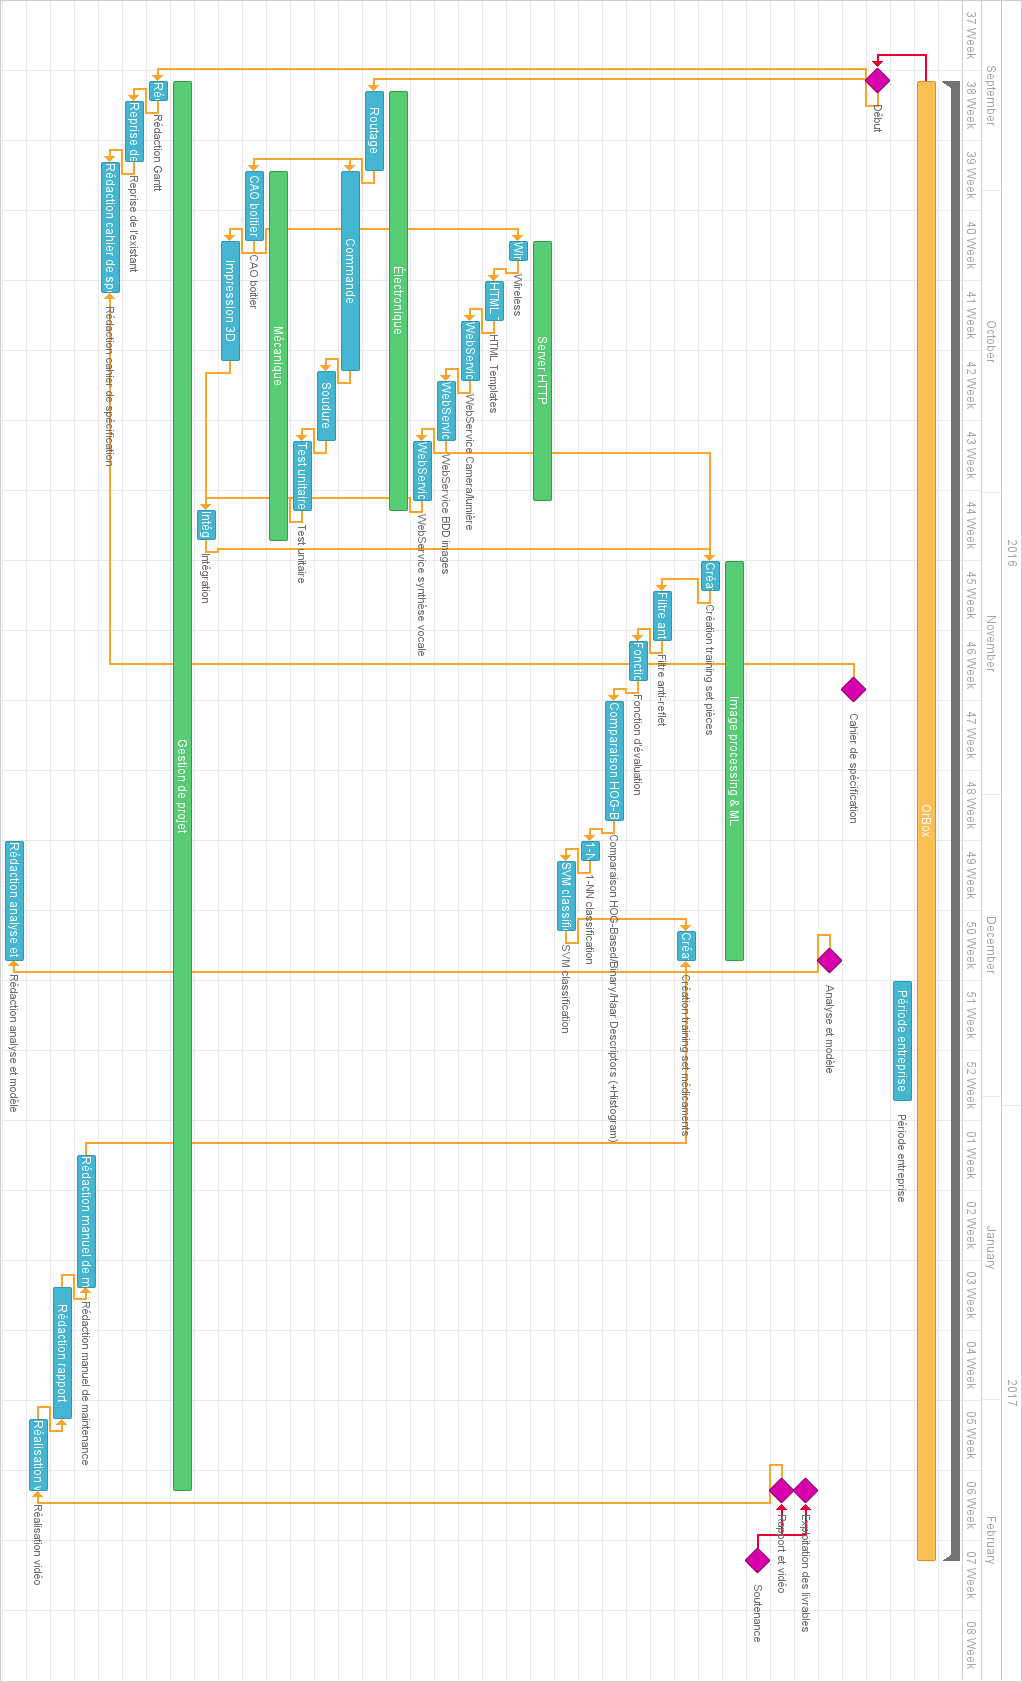
\includegraphics[width=\textwidth]{img/gantt.png}
}
\caption{Diagramme de Gantt}
\label{gantt}
\end{figure}

\section{Description des tâches}
%Vous devez dans cette partie réfléchir à la structuration de votre projet en tâches. Une tâche correspond ici à un ensemble de réalisations ayant une cohésion d'ensemble. Il peut s'agir de composants ou de fonctionnalités du système tels qu'identifiés dans les sections~\ref{sec:archi} et~\ref{sec:fonctions} mais le plus souvent, les tâches sont transversales aux fonctions et/ou aux composants. Ainsi, selon le point de vue adopté, un composant pourra effectuer plusieurs fonctions, une fonction pourra travailler sur plusieurs composants, etc. De même, la réalisation des interfaces homme/machine peut faire l'objet de tâches à part entière (améliore leur indépendance et les rend plus facilement évolutive) ou encore peut être intégrée à la réalisation de chaque composant auquel elles se rapportent.

%Ces tâches ne sont pas nécessairement indépendantes les unes des autres même si cela facilite souvent leur identification et permet de répartir plus facilement les charges. On indiquera également ici les tâches relatives à la gestion de projet (prise en mains de l'existant, bibliographie, rédaction du cahier de spécification, du rapport, de manuels techniques ou utilisateurs, mise en production et recette globale, etc. Chaque tâche doit être décrite précisément~:





\subsection{Image processing \& ML}

\subsubsection{Création training set pièces}

\begin{tabularx}{13cm}{lX}
    \toprule
        \textbf{Description} &
        Photographier avec la OrBox un premier set d'image composé de l'ensemble des pièces d'euro.
        L'intégralité des photos sera conservée afin de pouvoir tester différents réglages sur l'ensemble du processus d'Image Processing et de Machine Learning. \\
    \midrule
        \textbf{Livrables} &
        Base de données remplie. \\
    \midrule
        \textbf{Estimation de charge} &
        3 jours \\
    \midrule
        \textbf{Contraintes temporelles} &
        L'électronique doit être fonctionnelle et intégré dans le boitier.
        Les Web Services devront être fonctionnels. \\
    \bottomrule
\end{tabularx}

\subsubsection{Création training set médicaments}

\begin{tabularx}{13cm}{lX}
    \toprule
        \textbf{Description} &
        Photographier avec la OrBox un deuxième set d'image composé d'une sélection de médicament.
        Le but est de mesurer les capacités d'apprentissage des algorithmes mis en place. \\
    \midrule
        \textbf{Livrables} &
        Base de données remplie. \\
    \midrule
        \textbf{Estimation de charge} &
        3 jours \\
    \midrule
        \textbf{Contraintes temporelles} &
        Des résultats satisfaisants devront être sur le set des pièces dans un premier temps avant d'envisager la réalisation de cette tâche. \\
    \bottomrule
\end{tabularx}

\subsubsection{Filtre antireflet}

\begin{tabularx}{13cm}{lX}
    \toprule
        \textbf{Description} &
        Concevoir un filtre anti-reflet à ajouter au pipeline de preprocessing afin de limiter les déformations de l'objet suivant sa position sur la vitre.
        Le filtre vient en complément de la plaque diffusante. \\
    \midrule
        \textbf{Livrables} &
        Fonction logicielle OpenCV et les ressources associées pour être utilisé avec la Or-Box (image de la cartographie des reflets). \\
    \midrule
        \textbf{Estimation de charge} &
        3 jours \\
    \bottomrule
\end{tabularx}

\subsubsection{Fonction d'évaluation}
\label{TachEvalFun}

\begin{tabularx}{13cm}{lX}
    \toprule
        \textbf{Description} &
        Concevoir le bloc logiciel permettant de tester les algorithmes d'image processing et de machine learning mis en place.
        Cette fonction devra séparer le set d'image connu en deux sous-sets.
        Le premier servira à l'entraînement, le deuxième à l'évaluation.
        L'opération sera répétée plusieurs fois, différente paire de sous-sets sont crée.
        La performance finale de l'algorithme est la moyenne du taux de réussite sur chaque paire de sous-sets.
        Un rapport devra être généré. \\
    \midrule
        \textbf{Livrables} &
        Une fonction logicielle et sa documentation. \\
    \midrule
        \textbf{Estimation de charge} &
        4 jours \\
    \midrule
        \textbf{Contraintes temporelles} &
        Cette fonction doit être opérationnelle avant le développement des fonctionnalités de machine learning pour comparer les différentes méthodes de manière objective. \\
    \bottomrule
\end{tabularx}

\subsubsection{Comparaison HOG-Based/Binary/Haar Descriptors (+Histogram)}

\begin{tabularx}{13cm}{lX}
    \toprule
        \textbf{Description} &
        Implémenter les différents extracteurs de features, leurs différentes représentations associées (sérialisation des données pour OpenCV et pour DINet Viewer).
        Le but est de découvrir expérimentalement quels descripteurs est le plus pertinent pour notre application. La contrainte de performance du taux de reconnaissance de 90\% repose majoritairement sur cette partie.\\
    \midrule
        \textbf{Livrables} &
        Une fonction logicielle et sa documentation.
        La base de données remplie avec les différents descripteurs pour chaque pièce du set. \\
    \midrule
        \textbf{Estimation de charge} &
        10 jours \\
    \bottomrule
\end{tabularx}

\subsubsection{1-NN classification}

\begin{tabularx}{13cm}{lX}
    \toprule
        \textbf{Description} &
        Première méthode de classification assez naïve, 1-NN (voisin le plus proche).
        C'est une deuxième façon de mesurer la robustesse du descripteur choisi en plus de l'analyse visuelle faite avec DINet Viewer.
        \\
    \midrule
        \textbf{Livrables} &
        Fonction OpenCV et sa documentation. \\
    \midrule
        \textbf{Estimation de charge} &
        2 jours \\
    \bottomrule
\end{tabularx}

% subsection CVML (end)

\subsection{Server HTTP}

\begin{tabularx}{13cm}{lX}
    \toprule
        \textbf{Description} &
        Développement des différents web services qui respectent l'API défini en annexe \ref{annexe_api}.  \\
    \midrule
        \textbf{Livrables} &
        Le code sur GitHub + le wiki avec la procédure d'installation. \\
    \midrule
        \textbf{Estimation de charge} &
        18 jours \\
    \midrule
        \textbf{Contraintes temporelles} &
        La tâche doit être mené à bien avant la phase d'intégration. \\
    \bottomrule
\end{tabularx}

\subsection{Électronique}

\subsubsection{Routage}

\begin{tabularx}{13cm}{lX}
    \toprule
        \textbf{Description} &
        Réalisation du schéma électrique (choix des structures électronique, dimensionnement des composants). Réalisation du bon de commande. Routage du PCBs (prise en compte des problèmatiques de CEM, respect des contraintes de fabrication du sous-traitant).  \\
    \midrule
        \textbf{Livrables} &
        Un schéma électrique + un BOM + un Typon/Gerber \\
    \midrule
        \textbf{Estimation de charge} &
        6 jours \\
    \midrule
        \textbf{Contraintes temporelles} &
        Clotûre de la comptabilité de Polytech pendant le mois de novembre et décembre. \\
    \bottomrule
\end{tabularx}

\subsubsection{Commande}

\begin{tabularx}{13cm}{lX}
    \toprule
        \textbf{Description} &
        Cette tâche permet de modéliser le temps de réception de la commande des composants électroniques et de la sous-traitance du PCB sur le diagramme de Gantt.
        Un suivi régulier de l'avancement des commandes auprès de S. Beaufils devra être effectué.\\
    \midrule
        \textbf{Livrables} &
        L'ensemble des composants nécessaires à l'assemblage de la carte électronique. \\
    \midrule
        \textbf{Estimation de charge} &
        14 jours \\
    \midrule
        \textbf{Contraintes temporelles} &
        Clotûre de la comptabilité de Polytech pendant le mois de Novembre et décembre. \\
    \bottomrule
\end{tabularx}

\subsubsection{Soudure}

\begin{tabularx}{13cm}{lX}
    \toprule
        \textbf{Description} &
        Soudure des composants électroniques sur le PCB. \\
    \midrule
        \textbf{Livrables} &
        Carte électronique montée. \\
    \midrule
        \textbf{Estimation de charge} &
        5 jours \\
    \midrule
        \textbf{Contraintes matérielles} &
        Besoin des outils nécessaires à la soudure de composants CMS : binoculaire, flux de soudure, pâte à souder, pince brucelles. \\
    \bottomrule
\end{tabularx}

\subsubsection{Test unitaire}

\begin{tabularx}{13cm}{lX}
    \toprule
        \textbf{Description} &
        Tester chaque fonction électronique présente sur la carte (pour un total de quatre). \\
    \midrule
        \textbf{Livrables} &
        Une fiche de test rempli pour chaque fonction électronique testée. \\
    \midrule
        \textbf{Estimation de charge} &
        5 jours \\
    \midrule
        \textbf{Contraintes matérielles} &
        Besoin d'un minimum d'outils de mesures : oscilloscope, générateur de signal... \\
    \bottomrule
\end{tabularx}

% subsection Electronique (end)

\subsection{Mécanique}

\subsubsection{CAO boitier}

\begin{tabularx}{13cm}{lX}
    \toprule
        \textbf{Description} &
        Concevoir le boitier plastique de la OrBox en tenant compte des contraintes liées aux moyens de fabrication disponible. \\
    \midrule
        \textbf{Livrables} &
        Fichier CAD (en format STL) du boitier, dont l'imprimibalité a été testé avec Cura. \\
    \midrule
        \textbf{Estimation de charge} &
        5 jours \\
    \midrule
        \textbf{Contraintes temporelles} &
        Le routage de la carte électronique doit être fini avant la réalisation de cette tâche afin de pouvoir l'intégrer au boitier. \\
    \bottomrule
\end{tabularx}

\subsubsection{Impression 3D}

\begin{tabularx}{13cm}{lX}
    \toprule
        \textbf{Description} &
        Cette tâche permet de modéliser le temps d'impression auprès du service informatique de Polytech.
        Un suivi régulier de l'avancement de l'impression auprès de S. Beaufils devra être effectué.\\
    \midrule
        \textbf{Livrables} &
        Le boîtier imprimé. \\
    \midrule
        \textbf{Estimation de charge} &
        8 jours \\
    \bottomrule
\end{tabularx}

\subsubsection{Intégration}

\begin{tabularx}{13cm}{lX}
    \toprule
        \textbf{Description} &
        Effectuer le montage des différentes pièces mécaniques du boîtier, câbler la carte électronique à la batterie, au Raspberry Pi, aux LED et boutons. \\
    \midrule
        \textbf{Livrables} &
        Fiche de recette remplie. \\
    \midrule
        \textbf{Estimation de charge} &
        3 jours \\
    \bottomrule
\end{tabularx}

% subsection Mecanique (end)

\subsection{Gestion de projet}

\subsubsection{Rédaction Gantt}

\begin{tabularx}{13cm}{lX}
    \toprule
        \textbf{Description} &
        Découper le projet en tâche et les ordonnancer. \\
    \midrule
        \textbf{Livrables} &
        Le Gannt (voir Figure \ref{gantt}). \\
    \midrule
        \textbf{Estimation de charge} &
        2 jours \\
    \bottomrule
\end{tabularx}

\subsubsection{Reprise de l'existant}

\begin{tabularx}{13cm}{lX}
    \toprule
        \textbf{Description} &
        Prendre les schémas et documents du précédent projet, faire la liste des ressources réutilisables en l'état et mise à jour des autres. \\
    \midrule
        \textbf{Livrables} &
        Projet VisualParadigme et Diagramme SysML compléter et mis à jour. \\
    \midrule
        \textbf{Estimation de charge} &
        5 jours \\
    \bottomrule
\end{tabularx}

\subsubsection{Rédaction du cahier de spécification}

\begin{tabularx}{13cm}{lX}
    \toprule
        \textbf{Description} &
        Rédaction cahier de spécification, il doit permettre de lister précisément ce qui va être fait durant le projet et comment cela va être fait. \\
    \midrule
        \textbf{Livrables} &
        Ce rapport. \\
    \midrule
        \textbf{Estimation de charge} &
        10 jours \\
    \midrule
        \textbf{Contraintes temporelles} &
        Date limite de dépôt le 19 Novembre, tenir compte du temps de relecture par la MOA. \\
    \bottomrule
\end{tabularx}

\subsubsection{Rédaction du rapport "analyse et modèle"}

\begin{tabularx}{13cm}{lX}
    \toprule
        \textbf{Description} &
        Rédaction du rapport d'analyse et modèle, il doit expliquer en détail les choix et solutions mises en places pour la réalisation du projet. \\
    \midrule
        \textbf{Livrables} &
        Le rapport d'analyse et modèle. \\
    \midrule
        \textbf{Estimation de charge} &
        10 jours \\
    \midrule
        \textbf{Contraintes temporelles} &
        Date limite de dépôt le 18 décembre, tenir compte du temps de relecture par la MOA. \\
    \bottomrule
\end{tabularx}

\subsubsection{Rédaction du manuel de maintenance}

\begin{tabularx}{13cm}{lX}
    \toprule
        \textbf{Description} &
        Rédaction du manuel de maintenance. \\
    \midrule
        \textbf{Livrables} &
        Le manuel de maintenance. \\
    \midrule
        \textbf{Estimation de charge} &
        10 jours \\
    \midrule
        \textbf{Contraintes temporelles} &
        Date limite de dépôt le 7 février, tenir compte du temps de relecture par la MOA. \\
    \bottomrule
\end{tabularx}

\subsubsection{Rédaction rapport}

\begin{tabularx}{13cm}{lX}
    \toprule
        \textbf{Description} &
        Rédaction rapport de projet. \\
    \midrule
        \textbf{Livrables} &
        Le rapport de projet. \\
    \midrule
        \textbf{Estimation de charge} &
        10 jours \\
    \midrule
        \textbf{Contraintes temporelles} &
        Date limite de dépôt le 7 février, tenir compte du temps de relecture par la MOA. \\
    \bottomrule
\end{tabularx}

\subsubsection{Réalisation vidéo}

\begin{tabularx}{13cm}{lX}
    \toprule
        \textbf{Description} &
        Réalisation d'une vidéo de présentation du produit. Cadrage, prise de son et montage. \\
    \midrule
        \textbf{Livrables} &
        Le projet du logiciel de montage, les ressources associées et la vidéo exportée. \\
    \midrule
        \textbf{Estimation de charge} &
        5 jours \\
    \midrule
        \textbf{Contraintes temporelles} &
        Date limite de dépôt le 7 février, tenir compte du temps de relecture par la MOA. \\
    \bottomrule
\end{tabularx}



% subsection GestionDeProjet (end)